\documentclass[journal]{IEEEtran}
% ---------------------------------------------------------------------------
% Are the People of the Mahabharata Real? A Pre-Registered Record-Linkage Test
% against the Vedic Corpus.  IEEEtran journal style.
% ---------------------------------------------------------------------------
\usepackage[T1]{fontenc}
\usepackage[utf8]{inputenc}
\usepackage{lmodern}
\usepackage{amsmath,amssymb}
\usepackage{graphicx}
\usepackage{booktabs}
\usepackage{array}
\usepackage{multirow}
\usepackage{tabularx}
\usepackage{xcolor}
\usepackage{tikz}
\usetikzlibrary{positioning,arrows.meta,shapes.geometric}
\usepackage[hidelinks]{hyperref}
\usepackage{cite}

% Sanskrit transliteration (IAST) under pdfLaTeX
\DeclareUnicodeCharacter{1E5B}{\d{r}}   % ṛ
\DeclareUnicodeCharacter{1E5A}{\d{R}}   % Ṛ
\DeclareUnicodeCharacter{1E63}{\d{s}}   % ṣ
\DeclareUnicodeCharacter{1E62}{\d{S}}   % Ṣ
\DeclareUnicodeCharacter{1E47}{\d{n}}   % ṇ
\DeclareUnicodeCharacter{1E6D}{\d{t}}   % ṭ
\DeclareUnicodeCharacter{1E0D}{\d{d}}   % ḍ
\DeclareUnicodeCharacter{1E43}{\d{m}}   % ṃ
\DeclareUnicodeCharacter{1E25}{\d{h}}   % ḥ
\DeclareUnicodeCharacter{1E45}{\.{n}}   % ṅ
\DeclareUnicodeCharacter{015B}{\'{s}}   % ś
\DeclareUnicodeCharacter{015A}{\'{S}}   % Ś
\DeclareUnicodeCharacter{0101}{\={a}}   % ā
\DeclareUnicodeCharacter{0100}{\={A}}   % Ā
\DeclareUnicodeCharacter{012B}{\={\i}}  % ī
\DeclareUnicodeCharacter{012A}{\={I}}   % Ī
\DeclareUnicodeCharacter{016B}{\={u}}   % ū
\DeclareUnicodeCharacter{016A}{\={U}}   % Ū
\DeclareUnicodeCharacter{2264}{\ensuremath{\le}}
\DeclareUnicodeCharacter{2265}{\ensuremath{\ge}}

\newcommand{\MBh}{\textit{Mahābhārata}}
\definecolor{sblue}{HTML}{2A78D6}
\definecolor{sorange}{HTML}{EB6834}

\begin{document}

\title{Are the People of the \MBh{} Real?\\ A Pre-Registered Record-Linkage Test\\ Against the Vedic Corpus}

\author{Jithendra~Varma~Chamarthi%
\thanks{Paper 1 of the series \textit{Itihāsa Through Data}.}%
\thanks{J. V. Chamarthi is an independent researcher (e-mail: jithendra9367@gmail.com; ORCID: 0000-0001-9467-5612).}%
\thanks{Data, code, the pre-registration protocol with all amendments, and every intermediate result: doi:10.5281/zenodo.23875710.}}

\markboth{Itihāsa Through Data, Paper 1 --- Preprint, November 2026}{Chamarthi: Are the People of the Mahābhārata Real?}

\maketitle

\begin{abstract}
Whether the people of the \MBh{} existed is usually argued case by case, from belief or from silence.
We replace the argument with a test. Every person in the epic's main lineages and embedded stories ($n=107$)
was compared with every person in the older Vedic corpus as catalogued in the \textit{Vedic Index of Names and
Subjects} ($n=2{,}051$ person records). The method combines four published approaches: oral-tradition criticism
(Vansina, Henige) to justify the Vedic texts as an independent witness; Mykytiuk's identifying-mark criteria for
matching a textual person with an external attestation; Fellegi--Sunter probabilistic record linkage with
frequency-based weights to score the marks; and a Bayesian posterior mapped onto Mykytiuk's grades. A protocol fixing
assumptions, rules and five ``battle tests'' was committed before any result was seen; every later change is
recorded as a numbered amendment. The first version failed its false-positive test (1.3\% against a 1\% limit).
Version 3, which uses a clean digital transcription of the Index, requires the Vedic text to state the same kind of
relationship as the epic, and treats tribes and conflicting roles as disqualifying, passes all pre-set tests:
21 matches against at most 11 in 1,000 permutations ($p=0.001$), 0.48\% false positives over 219,343 wrong-name
pairs, and 7 of 9 known identities recovered. Against a full hand review it reaches 0.76 precision and 0.84 recall,
and 0.95 precision when only identity (not historicity) is judged. A blind second review agreed with the first on every
identity decision (Cohen's $\kappa=1.00$; $\kappa=0.77$ when legendary figures are separated), and every relationship on
which a verdict depends was checked against the Critical Edition. The results are asymmetric. The generation
\emph{after} the war is securely attested: Janamejaya Pārikṣita, his three brothers and his priest Indrota appear in
the Śatapatha Brāhmaṇa together with the same expiation episode the epic tells. Earlier Kuru figures are real Vedic
names re-arranged into a new genealogy, and Rigvedic tribes became brothers. The war generation itself---the
Pāṇḍavas, the Kauravas, Bhīṣma, Droṇa, Karṇa and Draupadī---has no independent attestation.
\end{abstract}

\begin{IEEEkeywords}
Record linkage, entity resolution, Fellegi--Sunter model, computational history, digital humanities, pre-registration,
Mahābhārata, Vedic literature, oral tradition, prosopography.
\end{IEEEkeywords}

% ===========================================================================
\section{Introduction}
\IEEEPARstart{T}{he} \MBh{}, the longest surviving epic, names hundreds of kings, priests and warriors and arranges
them in detailed genealogies. Whether these people existed is one of the most contested questions in South Asian
history. Public debate often reduces it to two positions: that the epic is a record of real events, or that it is
literature with no historical content. Scholarly work has been more careful but has proceeded case by case, without
an explicit, repeatable standard of evidence~\cite{brockington1998,hiltebeitel2001,witzel1995}.

This paper asks a narrower question that can be tested: \emph{which people of the \MBh{} can be identified, with
stated confidence, with people named in older and independent sources?} It does not ask whether the war happened,
when it happened, or whether the epic's story is true. Identity is a precondition for every one of those later
questions, and it is the one question for which a suitable independent witness exists.

That witness is the Vedic corpus. Its texts are older than the epic text; they were memorised with interlocking
recitation patterns that make them unusually stable; and they mention kings and priests incidentally, as patrons and
authorities in ritual manuals rather than as heroes of a narrative. Witzel described the Vedic texts as ``tape
recordings'' of their period that ``we can use as basis for judging the less strict tradition of the
Epics''~\cite{witzel1995}. This paper turns that remark into a procedure.

\subsection{Contributions}
\begin{enumerate}
\item A \textbf{combined identification method} that joins oral-tradition source criticism~\cite{vansina1985,henige1974},
Mykytiuk's identifying-mark criteria~\cite{mykytiuk2004,mykytiuk2009}, Fellegi--Sunter record linkage with
value-specific weights~\cite{fellegi1969,newcombe1959,christen2012,binette2022}, and Bayesian grading.
\item A \textbf{pre-registered protocol} with five battle tests---a permutation null, a large-scale false-positive test,
known-identity recall, parameter sensitivity, and clerical review---and a public record of every amendment, including
the failures that motivated them.
\item \textbf{Two reproducible datasets}: the epic's people coded only from the epic, and every person record in the Vedic
Index~\cite{macdonell1912} parsed automatically from the Cologne digital transcription~\cite{cdsl}.
\item A \textbf{double review} with inter-rater agreement and a verse-level check of the epic side against the
Critical Edition.
\item \textbf{Substantive findings}: a securely attested post-war court, a re-arranged pre-war genealogy, tribes turned
into kin, and an unattested war generation.
\end{enumerate}

% ===========================================================================
\section{Background and Related Work}

\subsection{The Texts and Their Relative Age}
The Ṛgveda is conventionally dated to the second half of the second millennium BCE; the later Saṃhitās and the
Brāhmaṇas, in which most named kings and priests appear, to the early first millennium BCE~\cite{witzel1995}.
The \MBh{} text took shape over several centuries around the turn of the Common Era, with older narrative
material~\cite{brockington1998,hiltebeitel2001}. Its Critical Edition, prepared at the Bhandarkar Oriental Research
Institute between 1933 and 1966, collated manuscripts across scripts and regions~\cite{bori1966}. Only relative order
matters here: the Vedic witnesses are older than the epic text.

Witzel's study of the Kuru state identifies the late Ṛgvedic and early post-Ṛgvedic Kuru realm as the setting
of the epic and reads the \MBh{} as a tale of conflict within the Kuru people, recited at the court of the post-war
king~\cite{witzel1995}. That reading predicts exactly the kind of overlap tested here: Vedic attestation of the Kuru
dynasty around the epic's frame. Sinha similarly reads the \MBh{} as the \textit{itihāsa} of the late-Vedic Kuru clan,
tracing how a historical tradition was built from the Ṛgvedic battle of the ten kings to Kurukṣetra~\cite{sinha2021}.
Both arguments are made by close reading rather than by a stated, repeatable test.

\subsection{Historicity of Persons in Ancient Texts}
The closest methodological model comes from biblical archaeology. Mykytiuk~\cite{mykytiuk2004} formalised when a
person named in the Hebrew Bible may be identified with a person named in a Northwest Semitic inscription. His
criteria require (i) authentic data, (ii) a matching setting in time and place, and (iii) enough identifying
marks---name, father's name, title, place, family---that the two cannot be different people. Identifications fall into
six grades: S (certain, because singular circumstances require it), 3 (virtually certain to reliable), 2 (reasonable but
uncertain), 1 (doubtful), 0 (no identification, lacking a clear basis) and D (disqualified)~\cite{mykytiuk2004,freelib2007}.
Three matching marks with a fitting setting support grade~3, two support grade~2, and a name alone is never sufficient. Mykytiuk revised several cases after new discoveries and the exposure of forgeries~\cite{mykytiuk2009}.
His method uses inscriptions only. India has no deciphered inscriptions before Aśoka (third century BCE), so a
direct application would identify nobody; the adaptation in this paper replaces the inscription with an older
orally transmitted text and justifies that substitution with oral-tradition criticism.

Statistical arguments about named individuals in ancient sources have also been made from name frequencies, most
prominently in Feuerverger's analysis of the Talpiot tomb~\cite{feuerverger2008}, which drew extensive critical
discussion. The present study uses name frequency only to weight evidence, not to assert identity.

\subsection{Oral Tradition and Genealogies}
Vansina's \textit{Oral Tradition as History}~\cite{vansina1985} sets out how orally transmitted material can serve
as historical evidence and how it changes in transmission. Henige's \textit{The Chronology of Oral
Tradition}~\cite{henige1974} documents a specific failure mode of oral genealogies: real names are retained while
relationships and sequences are merged, lengthened and re-ordered. Both shape this study: Vansina in judging the
Vedic corpus as a witness, Henige in interpreting what the matches show about the epic's genealogies.

\subsection{Record Linkage}
Computerised record linkage began with Newcombe and colleagues' linkage of vital records~\cite{newcombe1959}.
Fellegi and Sunter~\cite{fellegi1969} gave it a decision-theoretic foundation: each compared field contributes a
log-likelihood ratio $\log(m/u)$, where $m$ is the probability that the field agrees for a true match and $u$ the
probability that it agrees by chance; value-specific $u$ lets rare values count more than common ones. Christen's
monograph~\cite{christen2012} and the review by Binette and Steorts~\cite{binette2022} survey modern blocking,
comparison, classification and evaluation practice, including precision--recall evaluation and clerical review,
which this study adopts.

\subsection{Gap}
To the author's knowledge no prior study has matched the persons of the \MBh{} against the Vedic corpus
\emph{systematically}---every person against every person---with a stated, pre-registered decision rule and
validation tests. The nearest precedent is Raychaudhuri's \textit{Political History of Ancient India}~\cite{raychaudhuri1923},
which compared the epic and Vedic accounts of the Kuru kings by hand, arguing for instance that the Vedic Parikṣit
corresponds to the epic's second Parikṣit. Other treatments (the Vedic Index's own notes~\cite{macdonell1912},
Witzel~\cite{witzel1995}, Sinha~\cite{sinha2021}) likewise discuss selected kings. Computational work on the epic has
modelled its characters only \emph{inside} the text: Gultepe and Mathangi built character networks from word vectors and
recovered the Pāṇḍava--Kaurava division~\cite{gultepe2023}, but did not test any character against external evidence.
The present study is, to the author's knowledge, the first to combine these strands: a systematic, statistical and
pre-registered comparison of the epic's people with an older, independent corpus.

% ===========================================================================
\section{Materials}

\subsection{The Epic Side}
The epic dataset contains 107 people: the Kuru main line from Pratīpa to Śatānīka; the Pāṇḍavas, Kauravas and their
allies; the Yādavas; the Pañcāla house; and the principal figures of the embedded stories (the Bharata, Purūravas,
Yayāti and Māndhātṛ legends, the Uddālaka--Śvetaketu and Janaka--Yājñavalkya episodes, and others). For each person
the father, mother, siblings, spouses, children, teachers or priests, people or dynasty, and a role class (royal,
sage/priest, woman, other) were coded from the epic's own genealogies and episodes, chiefly Ādiparvan 1.57--1.90,
\emph{without consulting any Vedic match}. Indian naming practice is followed: a patronymic names the legal father
(e.g., Dhṛtarāṣṭra is Vaicitravīrya, ``son of Vicitravīrya'').

\subsection{The Vedic Side}
Macdonell and Keith's \textit{Vedic Index of Names and Subjects}~\cite{macdonell1912} catalogues the persons, peoples,
places and terms of the Vedic texts with their passages. Version 1 of this study parsed an optical-character-recognition
(OCR) text of the 1912 scan; versions 2 and 3 use the Cologne Digital Sanskrit Lexicon transcription~\cite{cdsl}, which
encodes 3,834 entries with marked headwords, diacritics and separated footnotes. Person records were selected
automatically (a role word such as king, priest or teacher; a kinship word; or a patronymic in the headword),
giving 2,051 records. For each record only the entry's own main text is used. \textbf{Every sentence that mentions the
Epic, the Purāṇas, the Rāmāyaṇa, the Harivaṃśa or Pargiter is deleted}, because the Index often reports what the
later tradition says and would otherwise leak the epic's genealogy into the supposedly independent witness.

% ===========================================================================
\section{Method}

\subsection{Assumptions}
Table~\ref{tab:assumptions} lists the assumptions on which a match's meaning depends. A4 and A7 are deliberately
conservative: a shared name is never evidence, and absence is never disproof.

\begin{table}[!t]
\caption{Stated Assumptions}
\label{tab:assumptions}
\centering\footnotesize
\begin{tabularx}{\columnwidth}{@{}lX@{}}
\toprule
& Assumption \\
\midrule
A1 & The Vedic texts as edited today are faithful to their early form (oral transmission with cross-checking recitations). \\
A2 & The Vedic texts are older than the epic text. \\
A3 & A king or priest named incidentally in a ritual text was a person of that period (identity then implies existence only to that extent). \\
A4 & A shared name alone is not evidence: the epic's poets knew the Vedic texts. \\
A5 & A patronymic names the legal father. \\
A6 & The Vedic Index lists the persons of the Vedic texts with their key passages. \\
A7 & Absence from the Vedic texts is not disproof: they are ritual, not historical, texts. \\
\bottomrule
\end{tabularx}
\end{table}

\subsection{Pipeline}
Fig.~\ref{fig:pipeline} summarises the procedure. Each step implements one published method.

\begin{figure}[!t]
\centering
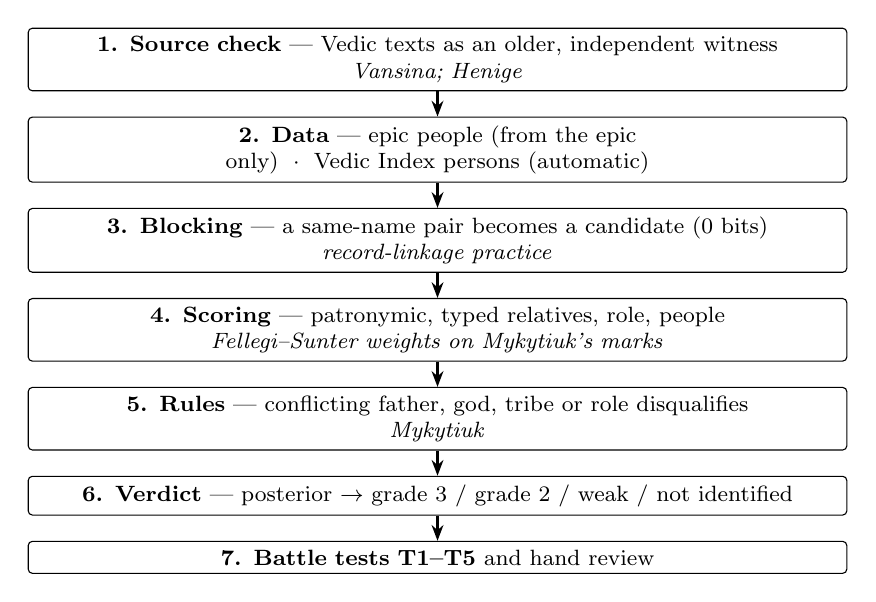
\begin{tikzpicture}[node distance=3.2mm, every node/.style={font=\footnotesize},
  box/.style={draw, rounded corners=1.5pt, align=center, text width=0.84\columnwidth, inner sep=3pt},
  arr/.style={-{Stealth[length=2mm]}, thick}]
\node[box] (a) {\textbf{1. Source check} --- Vedic texts as an older, independent witness\\ \textit{Vansina; Henige}};
\node[box, below=of a] (b) {\textbf{2. Data} --- epic people (from the epic only) \;$\cdot$\; Vedic Index persons (automatic)};
\node[box, below=of b] (c) {\textbf{3. Blocking} --- a same-name pair becomes a candidate (0 bits)\\ \textit{record-linkage practice}};
\node[box, below=of c] (d) {\textbf{4. Scoring} --- patronymic, typed relatives, role, people\\ \textit{Fellegi--Sunter weights on Mykytiuk's marks}};
\node[box, below=of d] (e) {\textbf{5. Rules} --- conflicting father, god, tribe or role disqualifies\\ \textit{Mykytiuk}};
\node[box, below=of e] (f) {\textbf{6. Verdict} --- posterior $\rightarrow$ grade 3 / grade 2 / weak / not identified};
\node[box, below=of f] (g) {\textbf{7. Battle tests T1--T5} and hand review};
\foreach \x/\y in {a/b,b/c,c/d,d/e,e/f,f/g} \draw[arr] (\x) -- (\y);
\end{tikzpicture}
\caption{The identification pipeline. Steps 1, 4 and 5 adapt published methods; step 7 is the validation design.}
\label{fig:pipeline}
\end{figure}

\subsection{Scoring Model}
Let an epic person $e$ and a Vedic record $v$ share a normalised name (transliteration- and OCR-insensitive; names
shorter than four letters must match exactly). For each identifying mark $k$ that is observed on both sides, the
Fellegi--Sunter weight is
\begin{equation}
w_k=\begin{cases}\log_2 \dfrac{m_k}{u_k} & \text{if the mark agrees,}\\[2mm]
\log_2 \dfrac{1-m_k}{1-u_k} & \text{if it conflicts,}\end{cases}
\end{equation}
and the evidence is $W=\sum_k w_k$ bits. The name itself contributes nothing (A4). The marks are:

\begin{itemize}
\item \textbf{Patronymic.} The second element of the Vedic name must \emph{begin} with the consonant skeleton of an
epic parent's name, as Sanskrit patronymics are formed on the parent's name (Pārikṣita, Vaicitravīrya, Prātipīya);
$m=0.85$, $u=0.01$. A patronymic matching no epic parent disqualifies.
\item \textbf{Typed relatives and associates.} An epic relative's name counts only if it occurs within twelve words of a
relation word of the \emph{same type} (Table~\ref{tab:relwords}); $m=0.80$, and $u$ is value-specific: the share of
Vedic entries containing that name, with $+1$ smoothing and a floor of 0.001~\cite{fellegi1969}.
\item \textbf{Role} (royal, sage/priest, woman); $m=0.90$, $u=0.30$.
\item \textbf{People or dynasty} named in the entry; $m=0.90$, $u$ frequency-based.
\end{itemize}

\begin{table}[!t]
\caption{Relation Words Required for a Typed Relative (Amendment 5)}
\label{tab:relwords}
\centering\footnotesize
\begin{tabularx}{\columnwidth}{@{}lX@{}}
\toprule
Epic relation & Vedic wording that counts \\
\midrule
Parent & son, daughter, descendant, father, mother, bore, patronymic \\
Child & son, daughter, father, mother, whose, his \\
Sibling & brother, brothers, sister \\
Spouse & wife, husband, queen, married, consort \\
Teacher/priest & priest, Purohita, pupil, teacher, taught, patron, officiated, sacrifice, court \\
\bottomrule
\end{tabularx}
\end{table}

With prior odds $\pi$ that a same-name candidate is the same person (main analysis $\pi=1/10$, allowing for
literary borrowing), the posterior probability of identity is
\begin{equation}
P(\text{same}\mid W)=\frac{\pi\,2^{W}}{1+\pi\,2^{W}}.
\end{equation}
Following Mykytiuk, $P\ge0.95$ is grade~3, $P\ge0.50$ grade~2, $P\ge0.05$ ``weak'' (Mykytiuk's grade~1, doubtful),
and below that ``not identified'' (grade~0); a disqualifying rule gives grade~D. Grade~S is not used: no Vedic attestation
is unique enough that singular circumstances force the identification.
Each epic person takes its best candidate.

\subsection{Disqualification Rules}
\begin{itemize}
\item[R2] A Vedic patronymic that matches no epic parent.
\item[R3] A Vedic namesake that is a god, demon or nymph where the epic has a human.
\item[R6] A Vedic entry whose opening describes a tribe or people (version 3).
\item[R7] Conflicting role classes on the two sides (version 3); Mykytiuk treats a conflicting mark as disqualifying.
\end{itemize}

\subsection{Battle Tests}
The protocol fixed five tests and their pass criteria before the first run:
\begin{itemize}
\item[T1] \textbf{Permutation null.} Relatives and parents are shuffled among epic people 1,000 times; the observed
number of grade~$\ge2$ matches must exceed the 99th percentile of the null.
\item[T2] \textbf{False positives.} Every epic person is scored against every Vedic person \emph{with a different name}
(ignoring blocking); fewer than 1\% of these wrong pairs may reach grade~$\ge2$.
\item[T3] \textbf{Known-identity recall.} Nine epic figures that standard scholarship identifies with Vedic figures
(Bharata, Yayāti, Purūravas, Māndhātṛ, Nala, Uddālaka, Śvetaketu, Yājñavalkya, Janaka); at least six must reach grade~$\ge2$.
\item[T4] \textbf{Sensitivity.} Prior odds 1:3 and 1:30, and each $m$ and $u$ moved by $\pm25\%$ (18 variants); a verdict is
robust only if unchanged across all.
\item[T5] \textbf{Clerical review.} Every grade~$\ge2$ match and every disqualification is read against the Vedic text.
\end{itemize}
If T1, T2 or T3 failed, results were to be reported as exploratory only.

\subsection{Pre-Registration and Amendments}
The protocol and frozen datasets were committed to version control before scoring. Seven amendments followed, each
committed with its reason (Table~\ref{tab:amend}); failed runs remain in the history. Amendments 4--5 and the version~3
rules were committed before the runs they govern.

\begin{table}[!t]
\caption{Amendments to the Protocol}
\label{tab:amend}
\centering\footnotesize
\begin{tabularx}{\columnwidth}{@{}clX@{}}
\toprule
\# & Trigger & Change \\
\midrule
1 & First run & Entry text only; delete sentences about the Epic/Purāṇas (circularity); stricter blocking \\
2 & T2 failed & Value-specific $u$ (frequency weights); anusvāra normalisation \\
3 & T2 diagnosis & Patronymic must \emph{start} with the parent's skeleton; an entry cannot name itself \\
4 & v1 precision 0.62 & Clean Cologne transcription replaces OCR \\
5 & v1 precision 0.62 & Typed relationships (Table~\ref{tab:relwords}) \\
6 & v2 parse check & Kinship words also mark a person record \\
v3 & v2 review & R6 tribe rule; R7 role-conflict rule \\
7 & CE check & Somaka's father and Arjuna's son corrected (data only) \\
\bottomrule
\end{tabularx}
\end{table}

% ===========================================================================
\section{Results}

\subsection{Battle Tests}
Table~\ref{tab:battle} reports the three versions. Version~1 failed T2. Versions~2 and~3 pass T1, T2 and T3.
Fig.~\ref{fig:null} shows the version~3 permutation null: 21 observed matches against a null mean of 5.8, a 99th
percentile of 9 and a maximum of 11 in 1,000 shuffles ($p=0.001$). Fig.~\ref{fig:versions} shows the false-positive
rate and agreement with the hand review across versions.

\begin{table}[!t]
\caption{Battle-Test Results by Version}
\label{tab:battle}
\centering\footnotesize
\begin{tabular}{@{}lccc@{}}
\toprule
Test (pass criterion) & v1 & v2 & v3 \\
\midrule
T1 observed / null 99th pct. & 24 / 13 & 26 / 12 & \textbf{21 / 9} \\
T1 $p$ & 0.001 & 0.001 & \textbf{0.001} \\
T2 false-positive rate ($<1\%$) & 1.30\% & 0.60\% & \textbf{0.48\%} \\
T2 wrong-name pairs & 207,801 & 219,343 & 219,343 \\
T3 known identities ($\ge6/9$) & 6 & 7 & \textbf{7} \\
T5 precision & 0.62 & 0.71 & \textbf{0.76} \\
T5 recall & 0.83 & 0.83 & \textbf{0.84} \\
T5 identity-only precision & --- & --- & \textbf{0.95} \\
\midrule
Verdict & \textcolor{sorange}{fail} & pass & \textbf{pass} \\
\bottomrule
\end{tabular}
\end{table}

\begin{figure}[!t]
\centering
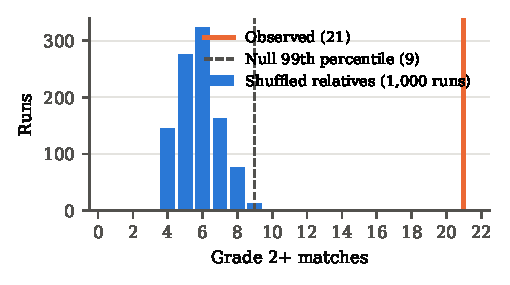
\includegraphics[width=\columnwidth]{figures/fig_null.pdf}
\caption{T1 permutation test, version 3. Bars: number of grade~$\ge2$ matches in each of 1,000 runs with relatives
shuffled among epic people. Line: the observed count with the true relatives.}
\label{fig:null}
\end{figure}

\begin{figure}[!t]
\centering
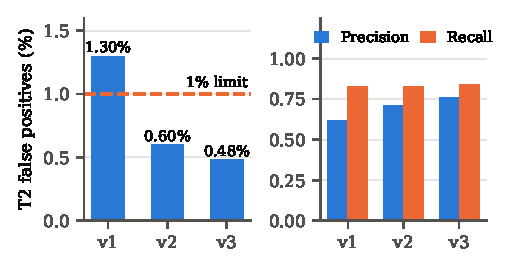
\includegraphics[width=\columnwidth]{figures/fig_versions.pdf}
\caption{Left: T2 false-positive rate by version against the pre-set 1\% limit. Right: precision and recall against
the hand review.}
\label{fig:versions}
\end{figure}

\paragraph*{Errors that remain} Of the 21 version~3 matches, 16 agree with the hand review. Four of the five
disagreements are correct identities of figures the Vedic texts treat as legendary or as a family name (Purūravas,
Yayāti, Viśvāmitra, Vasiṣṭha); counting identity alone, 20 of 21 are right. The single true error (Kuru) is a parsing
slip in which the entry Kuruśravaṇa was read as ``Kuru''. Three hand-confirmed links are missed (Parikṣit, Yājñavalkya,
Kalmāṣapāda) because the relation is stated in another entry or sentence. T4 flags 28 of the 107 automatic verdicts
as sensitive to the prior or to a $\pm25\%$ parameter shift; the hand review therefore decides the final grades.

\subsection{Critical Edition Check of the Epic Side}
Every epic relationship on which a verdict depends was checked against the BORI Critical Edition electronic
text~\cite{bori1966,gretil} (Table~\ref{tab:ce}). Two coding errors were found and corrected (Amendment~7): the Critical
Edition does not make Somaka the son of Sahadeva---the two are only listed together at 3.125.23, the filiation coming from
the Purāṇas---and Arjuna's son by Draupadī is Śrutakīrti. The first correction lowered Somaka from grade~3 to grade~2.
The check also strengthened one case: the epic's Baka Dālbhya episode names Dhṛtarāṣṭra \textit{vaicitravīryin} (9.40.1),
the same patronymic as the Vedic record in the same quarrel.

\begin{table}[!t]
\caption{Epic Relationships Checked Against the Critical Edition}
\label{tab:ce}
\centering\footnotesize
\begin{tabularx}{\columnwidth}{@{}X l c@{}}
\toprule
Relationship & CE & OK? \\
\midrule
Janamejaya, son of Parikṣit; brothers Śrutasena, Ugrasena, Bhīmasena & 1.3.1 & yes \\
Janamejaya's son Śatānīka by Vapuṣṭamā & 1.90.94 & yes \\
Pratīpa (Paryaśravas), son of Bhīmasena; sons Devāpi, Śaṃtanu, Bāhlīka & 1.90.44--46 & yes \\
Parikṣit, son of Abhimanyu & 1.36.17 & yes \\
Dhṛtarāṣṭra born in the field of Vicitravīrya & 1.57.95 & yes \\
Bharata, son of Duḥṣanta and Śakuntalā & 1.89.16 & yes \\
Yayāti, son of Nahuṣa; Purūravas, son of Ilā & 1.84.1; 1.70.16 & yes \\
Śakti, son of Vasiṣṭha, eaten by Kalmāṣapāda & 1.166.4--36 & yes \\
Āruṇi Pāñcālya; Śvetaketu Auddālaki & 1.3.20; 3.132.1 & yes \\
Māndhātṛ Yauvanāśva & 3.126.1 & yes \\
Indrota Śaunaka and Janamejaya & 12.146--148 & yes \\
Drupada = Yajñasena; Śikhaṇḍin, child of Drupada & 1.122.26; 1.57.104 & yes \\
Baka Dālbhya and Dhṛtarāṣṭra \textit{vaicitravīryin} & 9.40.1 & yes \\
\midrule
Somaka, son of Sahadeva & 3.125.23 & \textbf{no}$^{a}$ \\
Arjuna's son by Draupadī is Śrutakīrti & 1.90.82 & fixed$^{b}$ \\
\bottomrule
\multicolumn{3}{@{}p{0.95\columnwidth}@{}}{\scriptsize $^{a}$Only listed together; the filiation is Purāṇic. Somaka lowered to grade~2.
$^{b}$Coding error corrected; no verdict affected.}
\end{tabularx}
\end{table}

\subsection{Second Review and Inter-Rater Agreement}
To address the single-reviewer threat, a second reviewer judged 61 people blind: it received only the epic record and the
candidate Vedic entries, in shuffled order, with no automatic scores and no first-review verdicts, and applied the same
categories. The second reviewer was an AI model run separately from the analysis; a human Sanskritist review remains the
recommended next step. On the 37 people both reviewed (Table~\ref{tab:kappa}), the reviewers agreed on every identity
decision. All five category disagreements concern whether a correctly identified figure is historical or legendary
(Vyāsa, Kalmāṣapāda, Vasiṣṭha, Yayāti, Viśvāmitra), and all five grade disagreements are grade~3 versus grade~2, the second
reviewer being stricter each time. Disagreements were adjudicated conservatively: the lower grade, or ``same figure,
historicity disputed''.

\begin{table}[!t]
\caption{Agreement Between the Two Reviews ($n=37$)}
\label{tab:kappa}
\centering\footnotesize
\begin{tabular}{@{}lccl@{}}
\toprule
Level & Agree & $\kappa$ & Reading \\
\midrule
Same person? (accept/reject) & 37/37 & 1.00 & perfect \\
Identified / legendary / not & 32/37 & 0.77 & substantial \\
Exact grade & 22/37 & 0.52 & moderate \\
\bottomrule
\end{tabular}
\end{table}

\subsection{Identifications}
Table~\ref{tab:results} gives the adjudicated verdicts; Fig.~\ref{fig:bits} the evidence for the automatic matches.

\begin{table*}[!t]
\caption{Adjudicated Identifications of \MBh{} People in the Vedic Corpus (Two Reviewers; Conservative Adjudication)}
\label{tab:results}
\centering\footnotesize
\begin{tabularx}{\textwidth}{@{}>{\raggedright}p{2.9cm} >{\raggedright}p{4.3cm} X >{\raggedright\arraybackslash}p{2.4cm}@{}}
\toprule
Epic person & Vedic person (source) & Matching marks & Verdict \\
\midrule
Janamejaya & Janamejaya Pārikṣita (ŚB 13.5.4; AB 8.21) & Father Parikṣit; brothers Ugrasena, Bhīmasena, Śrutasena; priest Indrota; same expiation episode (ŚB 13.5.4.1 / \MBh{} 12.146--148) & Grade 3 \\
Ugrasena & Ugrasena Pārikṣitīya (ŚB 13.5.4.3) & Brother of Janamejaya, with Bhīmasena and Śrutasena & Grade 3 \\
Indrota Śaunaka & Indrota Daivāpa Śaunaka (ŚB 13.5.4.1) & Janamejaya's priest in the same episode & Grade 3 \\
Uddālaka; Śvetaketu & Uddālaka Āruṇi; Śvetaketu Āruṇeya & Father and son; Pañcāla setting & Grade 3 \\
Janaka & Janaka of Videha & Patron of Yājñavalkya & Grade 3 \\
Śakti & Śakti (Jaiminīya Br.) & Son of Vasiṣṭha; killed at the instigation of the Viśvāmitras & Grade 3 \\
\midrule
Śrutasena (and Bhīmasena) & The Pārikṣitīyas (ŚB 13.5.4.3) & Brothers of Janamejaya & Grade 2 \\
Bālhika & Bālhika Prātipīya (ŚB 12.9.3.3) & Son of Pratīpa; Kuru king & Grade 2 \\
Bharata & Bharata Dauḥṣanti (ŚB 13.5.4.11--14) & Son of Duḥṣanta; mother Śakuntalā & Grade 2 \\
Māndhātṛ & Māndhātṛ Yauvanāśva & Son of Yuvanāśva; king & Grade 2 \\
Yājñavalkya & Yājñavalkya & Teacher at Janaka's court & Grade 2 \\
Somaka & Somaka Sāhadevya (ṚV 4.15) & King; Sahadeva named with him in both (filiation not in the CE) & Grade 2 \\
Parikṣit & Parikṣit (AV 20.127.7--10) & Kuru king; son Janamejaya. Some read the hymn as about Agni & Grade 2 \\
Dhṛtarāṣṭra & Dhṛtarāṣṭra Vaicitravīrya (Kāṭhaka S.) & Same patronymic in the same Baka/Vaka Dālbhya quarrel (CE 9.40.1); possibly not a Kuru & Grade 2 \\
Śaṃtanu & Śaṃtanu (ṚV 10.98; Nirukta 2.10) & With Devāpi as priest; brotherhood only in the Nirukta & Grade 2 \\
Kṛṣṇa & Kṛṣṇa Devakīputra (ChU 3.17.6) & Mother Devakī; a pupil, no royal context & Grade 2 \\
\midrule
Vyāsa; Yayāti; Viśvāmitra; Vasiṣṭha; Kalmāṣapāda & Vyāsa Pārāśarya; Yayāti Nāhuṣa; Viśvāmitra; Vasiṣṭha; the Saudāsas & Same figures; reviewers split on historical vs legendary & Same figure, historicity disputed \\
Purūravas; Śakuntalā & Purūravas Aila; Śakuntalā & Same figures; mythical or a nymph in the Vedic texts & Same figure, legendary \\
\midrule
Devāpi & Devāpi Ārṣṭiṣeṇa (ṚV 10.98) & Vedic father Ṛṣṭiṣeṇa, epic father Pratīpa & D \\
Śatānīka & Śatānīka Sātrājita (ŚB 13.5.4.19) & Vedic father Satrājit, epic father Janamejaya & D \\
Pratīpa & Pratīpa Prātisatvana (AV Khila) & Different patronymic; possibly not a name & D \\
Śikhaṇḍin; Śakuni & Śikhaṇḍin Yājñasena; Saubala & Patronymic matches but a priest / a pupil & D (role) \\
Yadu; Pūru & Tribes (ṚV) & Rigvedic tribes; the epic makes them brothers & Tribe, not person \\
\midrule
\multicolumn{3}{@{}p{14.2cm}}{Bhīṣma, Pāṇḍu, Kuntī, Mādrī, Gāndhārī, Draupadī, Drupada, Dhṛṣṭadyumna, the five Pāṇḍavas, Duryodhana, Duḥśāsana, Karṇa, Droṇa, Aśvatthāman, Kṛpa, Abhimanyu, Vidura, Satyavatī, Jarāsandha, Śiśupāla, Virāṭa, Śalya, Ghaṭotkaca and others} & 0 (no attestation) \\
\bottomrule
\end{tabularx}
\end{table*}

\begin{figure}[!t]
\centering
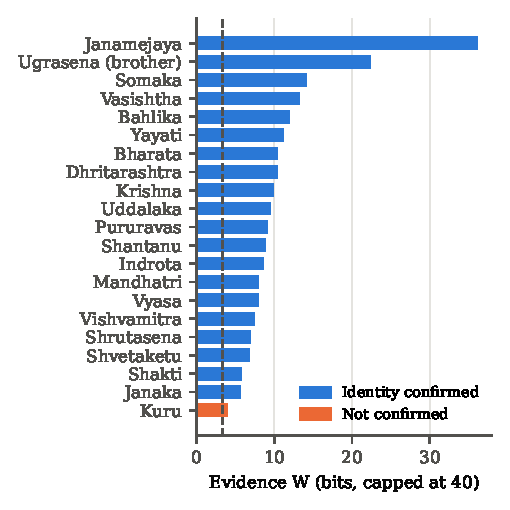
\includegraphics[width=\columnwidth]{figures/fig_bits.pdf}
\caption{Evidence (Fellegi--Sunter bits) for every automatic grade~$\ge2$ match in version 3, coloured by the hand
review: confirmed identity versus not confirmed. The dashed line is the grade-2 threshold at prior odds 1:10
($W=\log_2 10\approx3.3$ bits).}
\label{fig:bits}
\end{figure}

% ===========================================================================
\section{Discussion}

\subsection{An Asymmetric Record}
The attestations are not spread evenly over the epic's family tree. They concentrate in three places.

\textbf{The post-war court is securely attested.} Janamejaya Pārikṣita is the strongest identification in the study and
matches on six independent marks, including an entire episode: in both the Śatapatha Brāhmaṇa and the \MBh{}, the priest
Indrota performs a horse sacrifice to cleanse Janamejaya of killing a Brahmin. Witzel's reading of the epic as recited
at the court of the post-war Kuru king~\cite{witzel1995} is consistent with this result.

\textbf{The pre-war genealogy is real material re-arranged.} Bālhika, Śaṃtanu and Devāpi are real Vedic names, but the
relationships the epic gives them conflict with the Vedic record: Devāpi's father is Ṛṣṭiṣeṇa, not Pratīpa, and the
Ṛgveda shows Devāpi as Śaṃtanu's priest with ``no hint of relationship''~\cite{macdonell1912}. Śatānīka is a real king
but not Janamejaya's son. Rigvedic tribes (Yadu, Pūru, Turvaśa, Druhyu) become the sons of Yayāti. This is the pattern
Henige documents for oral genealogies: names survive, relationships are merged and re-ordered~\cite{henige1974}.

\textbf{The embedded stories rest on Vedic figures.} Uddālaka, Śvetaketu, Janaka and Śakti are identified at grade~3, and Bharata Dauḥṣanti, Somaka, Māndhātṛ Yauvanāśva and
Yājñavalkya at grade~2, several with father and associates. The epic drew its side
narratives from a known stock of Vedic persons and legends.

\subsection{The Silent Centre}
No member of the war generation---on either side---has an independent Vedic attestation. Under A7 this is not
disproof: the Brāhmaṇas are ritual manuals and may simply not mention them. But the silence is consistent, it falls
precisely on the generation the epic is about, and it contrasts with the attestation of the generations before and
after. The finding parallels other ancient epics in which a real place or dynasty frames heroes known only from the
poem.

\subsection{What the Method Contributes}
Two lessons generalise beyond this corpus. First, \emph{relationship type matters more than co-occurrence}: typed
relations halved the false-positive rate (1.30\%$\rightarrow$0.60\%) and raised precision. Second, \emph{circularity
is the main threat in historical linkage}: a reference work that reports a later tradition can leak that tradition into
the ``independent'' evidence, and must be filtered before scoring.

% ===========================================================================
\section{Threats to Validity}
\begin{itemize}
\item \textbf{Reviewers.} Two reviews agree on every identity ($\kappa=1.00$), but the second reviewer was an AI model,
not a human Sanskritist. A human expert review of the 37 adjudicated cases is the most important next step.
\item \textbf{Epic side.} Coded by one person; every relationship on which a verdict depends was checked against the
Critical Edition (Table~\ref{tab:ce}), but the remaining relationships were not.
\item \textbf{Not a blind test.} The author had seen a small hand-made register before the full run. Parameters were not
changed after the protocol, but the amendments were made in response to results; all are recorded.
\item \textbf{Identity, not existence.} A match shows the epic's person is the Vedic person. For Brāhmaṇa-period kings the
Vedic attestation is close to contemporary; for Ṛgvedic figures it may itself be legendary (A3).
\item \textbf{Coverage.} The Vedic Index is a 1912 reference work. Persons it omits cannot be found; Nala was not
recovered. Using the primary Vedic texts directly would extend coverage.
\item \textbf{Borrowing.} The epic's poets knew the Vedic texts. The method never counts a name, but borrowing of a name
together with its relations cannot be excluded.
\end{itemize}

% ===========================================================================
\section{Conclusion}
A pre-registered, battle-tested record-linkage method identifies seven people of the \MBh{} with Vedic persons at
grade~3 and eleven more at grade~2, with two reviewers agreeing on every identity. The results support a precise statement: the \MBh{} is framed around a real
late-Vedic Kuru court and draws on real Vedic figures, but it re-arranges their relationships, and its central war
heroes cannot be found outside the epic. The method, data and failures are documented so that the result can be
checked, contested and extended---to the Purāṇic king lists, to the Rāmāyaṇa, and to the later question of dating.

% ===========================================================================
\section*{Data and Code Availability}
The epic dataset, all scripts, the protocol with its seven amendments, the battle-test outputs, both reviews and the
adjudicated verdicts are released under CC BY 4.0 (code: MIT) on Zenodo, doi: 10.5281/zenodo.23875710~\cite{zenodo}.
Third-party texts are not redistributed; a script downloads them and verifies their checksums. The Vedic Index transcription is from the Cologne Digital Sanskrit Lexicon~\cite{cdsl}.

\section*{Use of AI Tools}
An AI assistant (Claude, Anthropic) was used to write analysis code, retrieve and check references, and draft text under
the author's direction. The author defined the research question, reviewed every identification, and takes full
responsibility for the content.

% ===========================================================================
\begin{thebibliography}{99}

\bibitem{witzel1995}
M. Witzel, ``Early Sanskritization: Origins and development of the Kuru state,''
\textit{Electronic Journal of Vedic Studies}, vol.~1, no.~4, Dec. 1995.

\bibitem{brockington1998}
J. Brockington, \textit{The Sanskrit Epics} (Handbook of Oriental Studies, Sect.~2, vol.~12).
Leiden, The Netherlands: Brill, 1998.

\bibitem{hiltebeitel2001}
A. Hiltebeitel, \textit{Rethinking the Mahābhārata: A Reader's Guide to the Education of the Dharma King}.
Chicago, IL, USA: Univ. of Chicago Press, 2001.

\bibitem{vansina1985}
J. Vansina, \textit{Oral Tradition as History}. Madison, WI, USA: Univ. of Wisconsin Press, 1985.

\bibitem{henige1974}
D. P. Henige, \textit{The Chronology of Oral Tradition: Quest for a Chimera}. Oxford, U.K.: Clarendon Press, 1974.

\bibitem{mykytiuk2004}
L. J. Mykytiuk, \textit{Identifying Biblical Persons in Northwest Semitic Inscriptions of 1200--539 B.C.E.}
(Academia Biblica, no.~12). Atlanta, GA, USA: Society of Biblical Literature, 2004.

\bibitem{mykytiuk2009}
L. J. Mykytiuk, ``Corrections and updates to `Identifying Biblical Persons in Northwest Semitic Inscriptions of
1200--539 B.C.E.','' \textit{Maarav}, vol.~16, no.~1, pp.~49--132, 2009.

\bibitem{fellegi1969}
I. P. Fellegi and A. B. Sunter, ``A theory for record linkage,'' \textit{J. Amer. Statist. Assoc.}, vol.~64, no.~328,
pp.~1183--1210, Dec. 1969, doi: 10.2307/2286061.

\bibitem{newcombe1959}
H. B. Newcombe, J. M. Kennedy, S. J. Axford, and A. P. James, ``Automatic linkage of vital records,''
\textit{Science}, vol.~130, no.~3381, pp.~954--959, Oct. 1959, doi: 10.1126/science.130.3381.954.

\bibitem{christen2012}
P. Christen, \textit{Data Matching: Concepts and Techniques for Record Linkage, Entity Resolution, and Duplicate
Detection}. Berlin, Germany: Springer, 2012, doi: 10.1007/978-3-642-31164-2.

\bibitem{binette2022}
O. Binette and R. C. Steorts, ``(Almost) all of entity resolution,'' \textit{Sci. Adv.}, vol.~8, no.~12,
Art.~no.~eabi8021, Mar. 2022, doi: 10.1126/sciadv.abi8021.

\bibitem{feuerverger2008}
A. Feuerverger, ``Statistical analysis of an archeological find,'' \textit{Ann. Appl. Statist.}, vol.~2, no.~1,
pp.~3--54, Mar. 2008, doi: 10.1214/08-AOAS99.

\bibitem{macdonell1912}
A. A. Macdonell and A. B. Keith, \textit{Vedic Index of Names and Subjects}, 2 vols. London, U.K.: John Murray, 1912.

\bibitem{cdsl}
Cologne Digital Sanskrit Dictionaries, ``The Vedic Index of Names and Subjects (VEI),'' Institute of Indology and
Tamil Studies, University of Cologne. [Online]. Available: https://www.sanskrit-lexicon.uni-koeln.de/
(transcription file \texttt{v02/vei/vei.txt}, \texttt{sanskrit-lexicon/csl-orig}).

\bibitem{zenodo}
J. V. Chamarthi, ``Are the People of the Mahābhārata Real? Data, code and protocol for a pre-registered record-linkage
test against the Vedic corpus,'' Zenodo, 2026 (all versions), doi: 10.5281/zenodo.23875710.

\bibitem{raychaudhuri1923}
H. C. Raychaudhuri, \textit{Political History of Ancient India: From the Accession of Parikshit to the Extinction of the
Gupta Dynasty}. Calcutta, India: Univ. of Calcutta, 1923.

\bibitem{sinha2021}
K. Sinha, \textit{From Dāśarājña to Kurukṣetra: Making of a Historical Tradition}. New Delhi, India: Oxford Univ.
Press, 2021.

\bibitem{gultepe2023}
E. Gultepe and V. Mathangi, ``A quantitative social network analysis of the character relationships in the
Mahabharata,'' \textit{Heritage}, vol.~6, no.~11, 2023, doi: 10.3390/heritage6110366.

\bibitem{freelib2007}
``Identifying Biblical Persons in Northwest Semitic Inscriptions of 1200--539 B.C.E.'' (book review), The Free Library,
2007. [Online]. Available: https://www.thefreelibrary.com/ (record a0166433699)

\bibitem{gretil}
Bhandarkar Oriental Research Institute, \textit{Mahābhārata}, electronic text based on M. Tokunaga \textit{et~al.}, rev.
J. Smith, 1999; Göttingen Register of Electronic Texts in Indian Languages (GRETIL). [Online]. Available:
https://gretil.sub.uni-goettingen.de/

\bibitem{bori1966}
V. S. Sukthankar \textit{et~al.}, Eds., \textit{The Mahābhārata, for the First Time Critically Edited}, 19 vols.
Poona, India: Bhandarkar Oriental Research Institute, 1933--1966.

\end{thebibliography}

\end{document}
